\section{Data Perspective: Abundant States}
\label{sec:data}

Section~\ref{sec:one-shot} showed that One-Shot OPD recovers much of full-data OPD's gain robustly. This section asks \textit{why training on a single query produces such a large gain, and whether the same explanation also covers the cases where n-shot OPD can match full-data OPD}. \footnote{The runs analyzed here and in Section~\ref{sec:algorithm} optimize the sampled-token advantage of Eq.~\ref{eq:token-advantage}, rather than the top-\(k\) advantage used by the mathematics runs of Section~\ref{sec:one-shot}, so their absolute accuracies differ slightly from those reported there. Every comparison below is between runs that share this form.}

\begin{tcolorbox}[takeawaysbox]
\begin{itemize}[topsep=0pt, partopsep=0pt, leftmargin=12pt, itemsep=0pt]
    \item \textbf{One query already reaches a large part of the full-data state space.}
    What OPD consumes is primarily states rather than queries. In practice, repeated rollouts from a single query can reach \(71.5\%\) state coverage, with most of it within the first \(100\) steps.

    \item \textbf{Diverse but few queries reach sufficient states and rival full-data performance.} Adding semantically distinct queries raises both state coverage and validation accuracy, and 16 queries already match full-data OPD. The value of an extra example lies in whether it covers states missed by earlier ones.
\end{itemize}
\end{tcolorbox}

\subsection{State Coverage of One-Shot OPD}
% \subsection{One Query Already Reaches \(71.5\%\) of the Full-Data State Space}
\label{sec:state-coverage}

\paragraph{Setup.}
OPD trains on states rather than queries. A query \(x\) and a sampled response \(y\) produce one state \(s=(x,y_{<i})\) at every token position \(i\), each paired with a target distribution from the teacher. With \(64\) rollouts per update, even a single query yields tens of thousands of supervised states, so query count can substantially understate the amount of supervision available to OPD.

\begin{tcolorbox}[examplebox, title={Hypothesis}]
\small
A single query can provide enough supervision to recover most of full-data OPD's gain if its rollouts cover a broad part of the state space visited by full-data OPD.
\end{tcolorbox}

To test this hypothesis, we measure the breadth rather than the raw number of visited states, since every generated token creates a distinct prefix. We call this measure \emph{state coverage}: we represent states in a shared representation space, partition that space into clusters, and report the fraction reached by a setting's rollouts.
\begin{itemize}[topsep=1pt, partopsep=0pt, leftmargin=13pt, itemsep=2pt, parsep=0pt]
    \item \textbf{Representation.} We represent each state by its \emph{teacher signature} \(h_T(s)\), the teacher's final-layer hidden vector at the state's last token.
    \item \textbf{Reference space.} We pool states visited by full-data OPD over its entire run on DAPO-Math-17K, sampling \(8\) uniformly spaced positions from each rollout. A held-out portion of these rollouts takes no part in defining the clusters and is measured as a setting of its own, \emph{full data (held-out)}.\footnote{Three of every five collected rollouts form the pool; the other two are the held-out setting, so it is what full-data OPD reaches on a fresh sample under the same budget.}
    \item \textbf{Clusters.} After PCA, \(K\)-means partitions the reference signatures into \(K=200\) clusters. Each state falls in the nearest one, denoted \(c(s)\).
\end{itemize}
The \emph{state coverage} of a set of states \(S\) is then the fraction of the \(K\) clusters it reaches:
\begin{equation}
    \mathrm{Cov}(S)
    =
    \frac{1}{K}
    \left|
    \left\{\,c(s)\;:\;s\in S\,\right\}
    \right|.
    \label{eq:state-coverage}
\end{equation}
Coverage records which clusters a setting reaches, not how often it visits them. We fit the clusters once and measure every setting over the same \(300\) steps. Full data (held-out) reaches \(100\%\) on this budget, so the top of the scale is a level full-data OPD attains rather than a maximum the construction guarantees. Appendix~\ref{app:state-coverage} gives the construction and schedule, and shows that the comparisons below are stable across choices of \(K\), reference set, and state positions.

\paragraph{One-shot OPD reaches \(71.5\%\) of the state space.}
\begin{figure}[t]
  \centering
  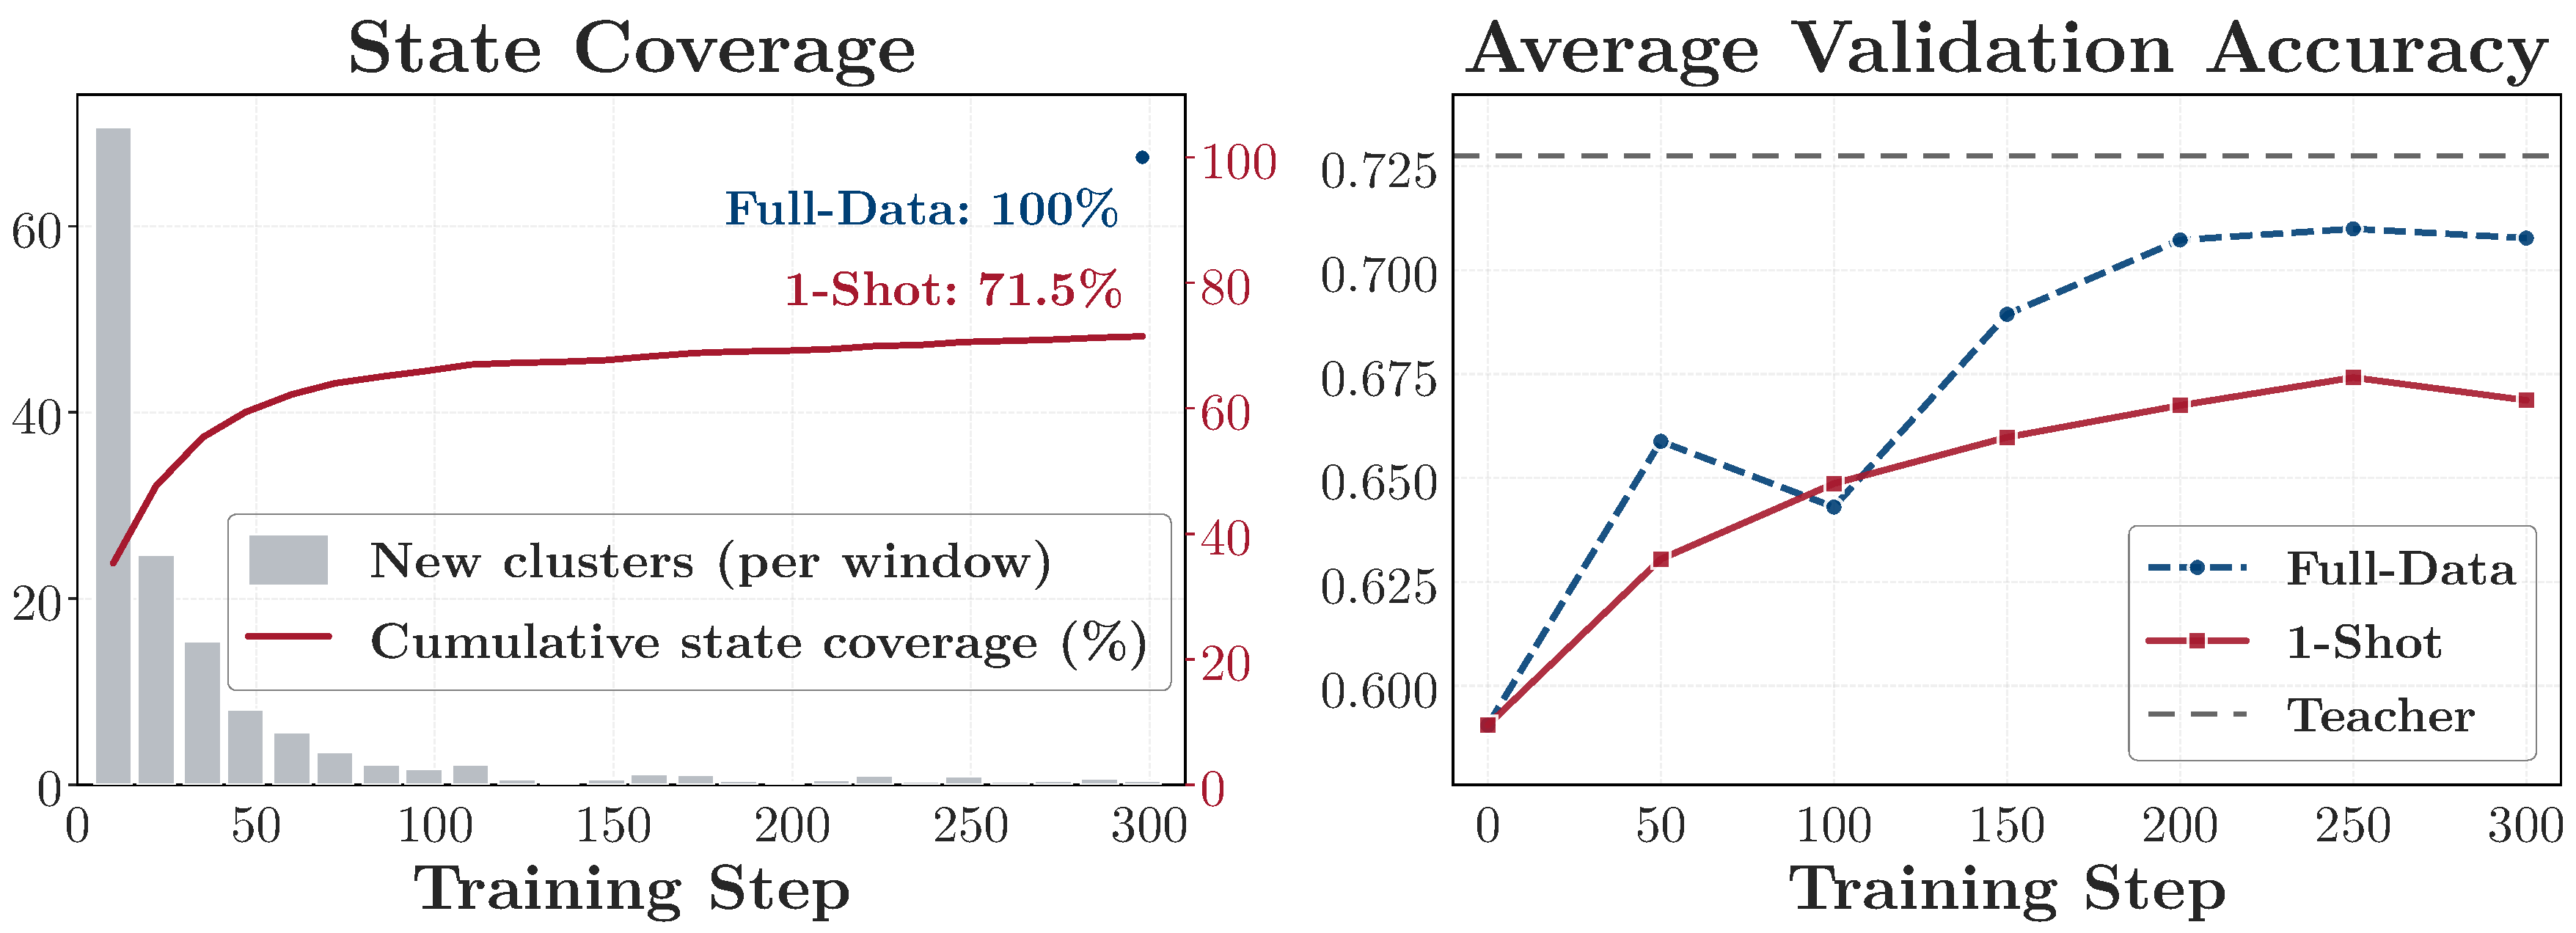
\includegraphics[width=0.75\linewidth]{figures/4_state_coverage_oneshot.pdf}
  \caption{
    State coverage and validation accuracy of one-shot OPD on the medium query, against full-data OPD. Coverage is measured against the state space full-data OPD reaches, which is therefore the \(1.0\) level rather than a separate curve.
  }
  \label{fig:state-coverage}
\end{figure}
Figure~\ref{fig:state-coverage} shows that one-shot OPD reaches \(71.5\%\) state coverage by step \(300\). Most of this coverage appears early: the run reaches \(65.9\%\) by step \(100\), then adds only \(5.6\) percentage points over the next \(200\) steps. Repeated rollouts from the same query therefore continue to discover new clusters, but at a sharply diminishing rate.
The same run raises validation accuracy from \(59.1\) to \(66.9\), compared with \(70.8\) for full-data OPD at step \(300\). These results show the same pattern on the data side: a single query already covers most of the state-space clusters reached by full-data OPD and produces a substantial validation gain. One-shot OPD is therefore small in query count, yet broad in the supervision it generates.

\subsection{Diversity Expands State Coverage}
% \subsection{Diverse Data Can Reach More States and Train a Better Student}
\label{sec:state-diversity}

The analysis above shows that one query already reaches most of the full-data state space, but it leaves the causal question open: a run that trains well might simply visit more states along the way, with the extra states doing none of the work. We therefore ablate state coverage directly, varying how many distinct states the training data reaches while holding the rest of the setup fixed.

\paragraph{Setup.}
We raise data diversity from two directions, each with its own control.
\textbf{(i) Response diversity (off-policy).} We sample \(64\) trajectories once from the initial student on the one-shot query and keep that pool fixed, which also removes a confound of on-policy training, where the states keep changing as the student does. Nested subsets retain \(1\), \(4\), \(16\), or all \(64\) trajectories, and the retained ones are repeated to fill each batch of \(64\). Every condition shares the query, the batch size, and the optimization budget, so the number of distinct trajectories, and hence of states, is the only quantity that changes.
\textbf{(ii) Query diversity (on-policy).} These runs instead change the query set, and all follow the mathematical configuration. Starting from the medium query used by one-shot OPD, we build 4- and 16-shot sets by clustering DAPO-Math-17K with BGE-M3~\citep{chen2024bge} and taking one representative per semantic cluster, so each query added to the ladder is semantically distinct from those already in it, and we compare these sets with full-data OPD.
We report validation accuracy for every run, and state coverage for the on-policy ones, where the rollouts are those the student actually generates during training. Off-policy scores are averaged over the five evaluation checkpoints from step \(300\) to \(500\). On the coverage side, the full-data bar is the held-out split that sets the \(100\%\) ceiling.

\begin{figure}[t]
  \centering
  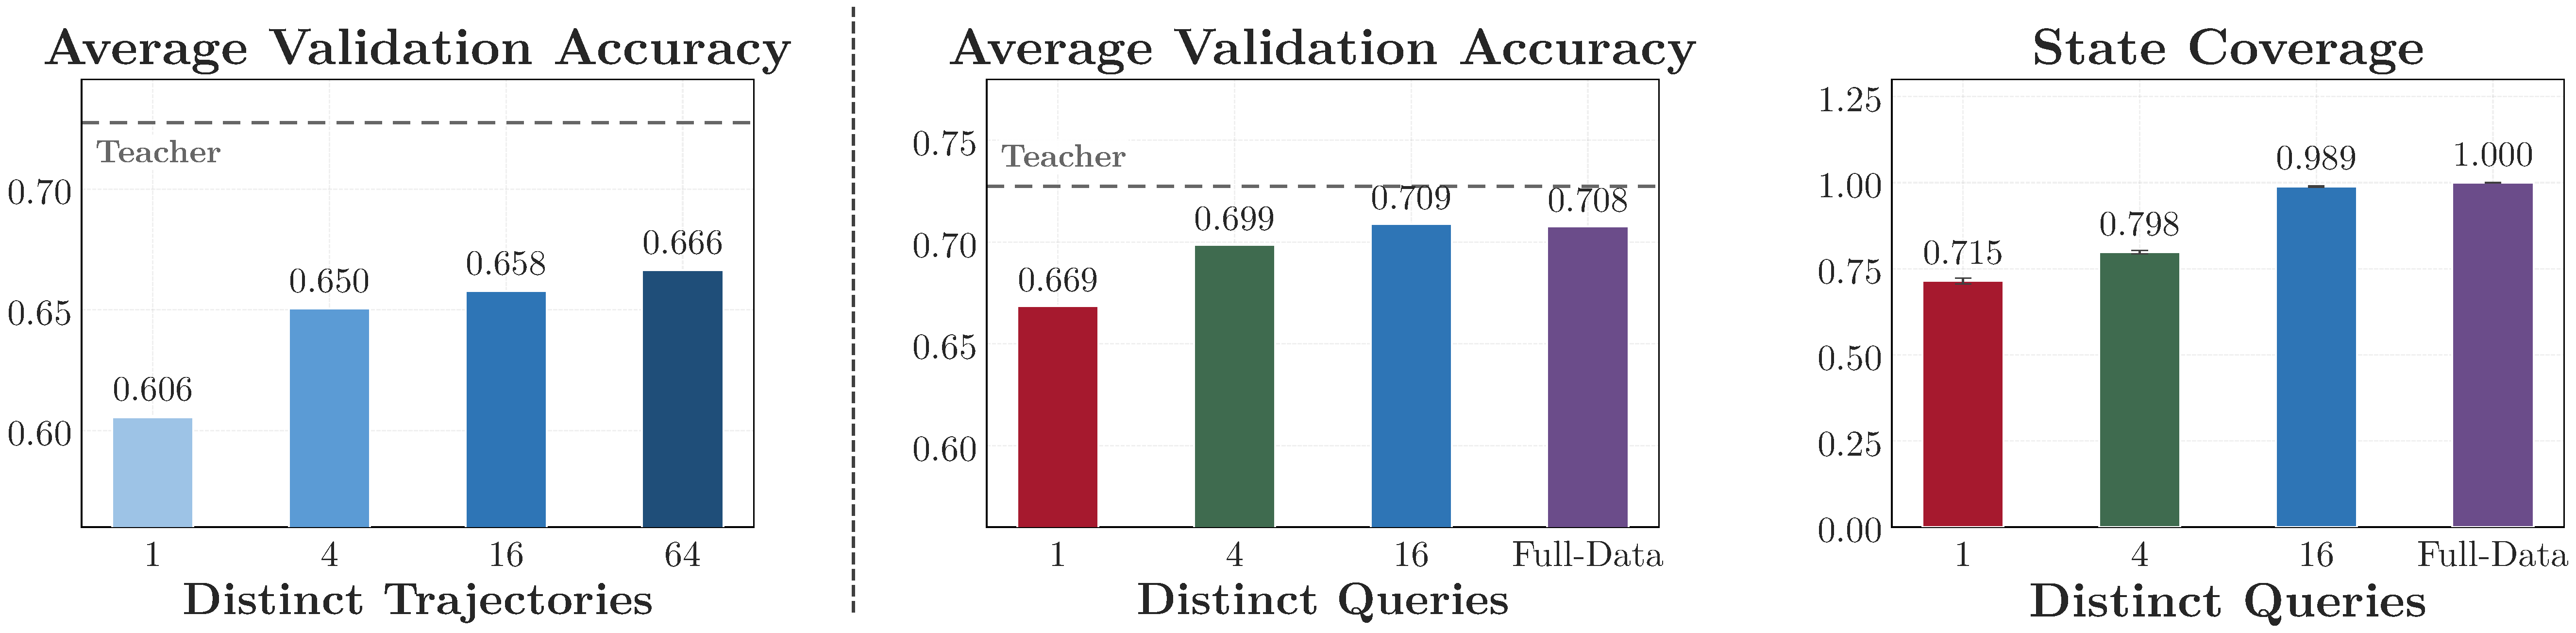
\includegraphics[width=\linewidth]{figures/4_state_diversity.pdf}
    \caption{
    Validation accuracy and state coverage as the training data is made more diverse, on the response side by off-policy training on distinct trajectories and on the query side by on-policy training on distinct queries.}
  \label{fig:state-diversity}
\end{figure}

\paragraph{Data diversity is state diversity, and a few queries match full-data OPD.}
Figure~\ref{fig:state-diversity} shows off-policy validation accuracy rising monotonically with the number of distinct trajectories. Everything else is held fixed, so the only thing the extra trajectories add is states. The on-policy runs reach the same conclusion from the query side. Semantically distinct queries raise validation accuracy until 16 of them match full-data OPD, and they match it on state coverage at the same point, which rises from \(71.5\%\) for one query to \(98.9\%\) for 16. Every query on the ladder is a new semantic cluster, so it raises diversity and count together, and two controls in Appendix~\ref{app:fixed-count-diversity} separate them: holding the count at 16, drawing those queries from 16 semantic clusters rather than from one raises state coverage and validation accuracy sharply, whereas the order in which the student trains on a fixed query set does not matter. What an added query is worth is therefore set by whether it reaches new states, and a few diverse queries already reach nearly all the states full-data OPD does.